\chapter{Proposed Approach}
\label{chap:approach}

This chapter presents the CORAL methodology. We first re-cap the conceptual two-stage architecture as introduced in FYP-1 and then present the full five-stage pipeline as deployed in FYP-2, with each stage given its own section. Each algorithmic component is presented with formal notation, pseudo-code, and a worked example. The implementation, deployment, and evaluation of this approach are deferred to Chapter \ref{chap:implementation}.

\section{From the FYP-1 Generate-and-Refine Concept to the Deployed Pipeline}
\label{sec:concept-to-pipeline}

\subsection{Conceptual Architecture (FYP-1)}
The original CORAL conceptual architecture, shown in Figure \ref{fig:coral-architecture-iter1} (Chapter \ref{chap:introduction}), framed the system as a two-stage \emph{Generate-and-Refine} pipeline:

\begin{itemize}
 \item \textbf{Stage 1 -- Multi-model Hypothesis Generation:} an ensemble of pre-trained ASR models (Whisper Large/Medium/Small + Wav2Vec2-XLSR Urdu) processes the audio and emits one confidence-annotated hypothesis per model.
 \item \textbf{Stage 2 -- Instruction-Guided Correction:} an instruction-tuned LLM (Alif-1.0-8B-Instruct) consumes the hypotheses and emits a single corrected transcript.
\end{itemize}

Iteration 1 implemented Stage 1 in full, established the baseline (Whisper-Large at 17.76\% WER on a 10-clip read-speech test set), and validated that architecture-specific confidence extraction was feasible. Iteration 2 then implemented the LLM stage but, when evaluated on real ASR output rather than synthetic hypotheses, exposed three practical problems: (i) confidences from heterogeneous architectures lived on incompatible scales, making cross-model arbitration unreliable; (ii) Arabic--Urdu Unicode conflation produced apparent disagreements where models had in fact agreed phonetically; and (iii) word-boundary disagreement was systematically misinterpreted by the LLM as substitution or deletion errors. These findings motivated the redesign described next.

\subsection{Deployed Five-Stage Pipeline (FYP-2)}
\label{ssec:deployed-pipeline}

The deployed system reorganises the conceptual two-stage architecture into five stages, indexed Stage 0 through Stage 4:

\begin{itemize}
 \item \textbf{Stage 0 -- Urdu Text Normalisation.} Strips diacritics, applies the seven canonical Arabic-to-Urdu character substitutions, removes tatweel and invisible characters, strips punctuation, and removes ASCII letters and digits.
 \item \textbf{Stage 1 -- Weighted Split-Merge-Aware Alignment.} Aligns each companion-model hypothesis to the source-model hypothesis using weighted word-level Levenshtein distance, then runs a secondary character-level alignment to classify each chunk as SAME/SPLIT/MERGE/NOISE.
 \item \textbf{Stage 2 -- OOV Detection and Candidate Ranking.} Flags out-of-vocabulary tokens via a dual criterion (model disagreement + frequency cutoff), retrieves candidates from a BK-tree, and ranks them using bi/tri-gram corpus context.
 \item \textbf{Stage 3 -- Consensus Voting and OOV Substitution.} Applies position-wise majority voting across companion models with conservative tie-breaking; OOV-flagged positions are replaced by the top-ranked candidate from Stage 2.
 \item \textbf{Stage 4 -- LLM Refinement.} Sends the voted transcript, the original raw source hypothesis, and structured alignment metadata to a commercial frontier LLM (Gemini, Claude Sonnet, or GPT-4o through OpenRouter) for fluency restoration, code-switching recovery, and named-entity handling.
\end{itemize}

The five-stage pipeline is illustrated in Figure \ref{fig:coral-pipeline}.

\begin{figure}[h]
 \centering
 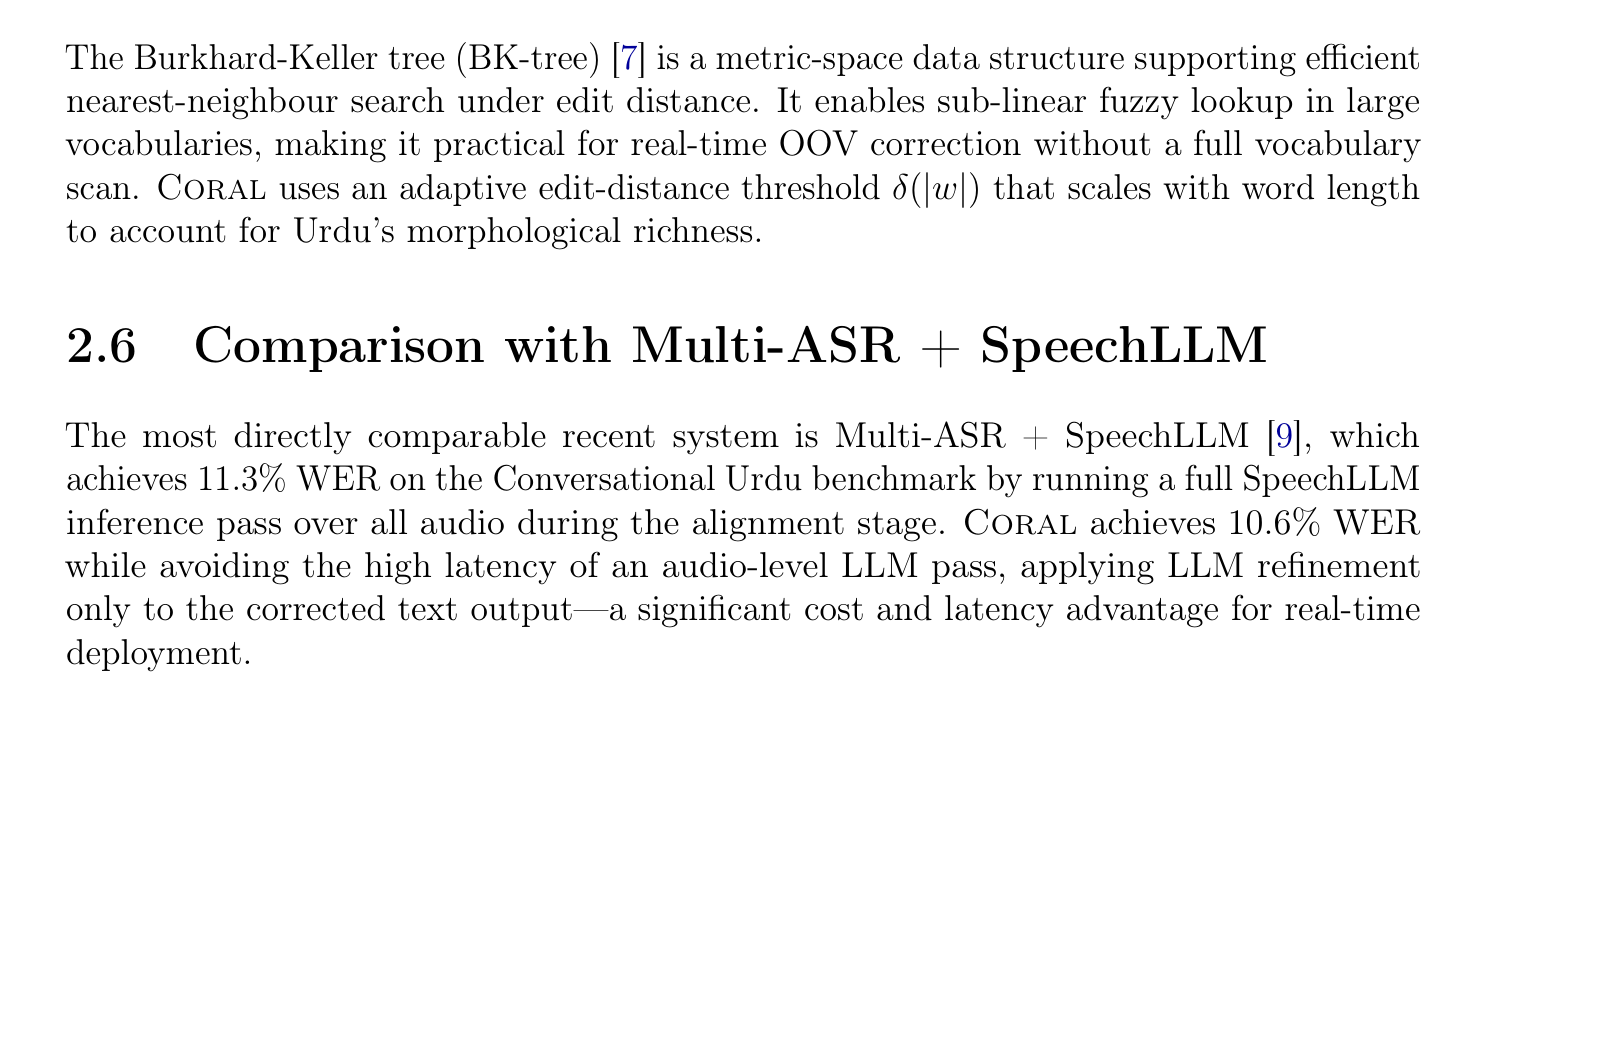
\includegraphics[width=0.95\textwidth]{ThesisFigs/fyp2_pipeline.png}
 \caption{The deployed CORAL pipeline (FYP-2). Stages 0--3 are server-side Python (FastAPI). Stage 4 is the LLM refinement layer invoked from the React front-end.}
 \label{fig:coral-pipeline}
\end{figure}

We now describe each stage in detail.

\begin{figure}[htbp]
    \centering
    \resizebox{0.98\textwidth}{!}{%
    \begin{tikzpicture}[every node/.style={font=\small\sffamily}, node distance=6mm]
      % external entity: audio
      \node[coral/entity, minimum width=20mm] (audio) at (0, 0) {Audio\\input};
      % ensemble of ASR backends
      \node[coral/data, minimum width=30mm] (m1) at (3.0,  1.5) {Seamless-Large};
      \node[coral/data, minimum width=30mm] (m2) at (3.0,  0.5) {Whisper-Large-v3};
      \node[coral/data, minimum width=30mm] (m3) at (3.0, -0.5) {Whisper-Medium};
      \node[coral/data, minimum width=30mm] (m4) at (3.0, -1.5) {Wav2Vec2-Urdu};
      \node[coral/sublabel] at (3.0, 2.2) {ASR ensemble (Kaggle GPU notebooks)};
      % stages
      \node[coral/stage, minimum width=24mm] (st0) at (6.5, 0)  {\textbf{Stage 0}\\Normalise};
      \node[coral/stage, minimum width=26mm] (st1) at (9.3, 0)  {\textbf{Stage 1}\\Split-Merge\\Alignment};
      \node[coral/stage, minimum width=26mm] (st2) at (12.2, 0) {\textbf{Stage 2}\\OOV Detect\\\& Rank};
      \node[coral/stage, minimum width=26mm] (st3) at (15.1, 0) {\textbf{Stage 3}\\Consensus\\Voting};
      \node[coral/llm,   minimum width=28mm] (st4) at (18.1, 0) {\textbf{Stage 4}\\LLM\\Refinement};
      % output
      \node[coral/entity, minimum width=22mm] (out) at (21.0, 0) {Corrected\\transcript};
      % data tier
      \node[coral/api, minimum width=70mm, align=center] (data)
        at (12.2, -2.2) {Data tier: BK-tree (joblib) + bi/tri-gram tables (DuckDB Parquet)};
      \node[coral/sublabel] at (12.2, -2.9) {downloaded from HuggingFace bucket on startup};
      % arrows (audio -> backends)
      \foreach \t in {m1,m2,m3,m4} \draw[coral/arrow] (audio.east) -- (\t.west);
      % backends -> stage 0
      \foreach \t in {m1,m2,m3,m4} \draw[coral/arrow] (\t.east) -- (st0.west);
      % stage chain
      \draw[coral/arrow] (st0) -- (st1);
      \draw[coral/arrow] (st1) -- (st2);
      \draw[coral/arrow] (st2) -- (st3);
      \draw[coral/arrow] (st3) -- (st4);
      \draw[coral/arrow] (st4) -- (out);
      % data tier dependency
      \draw[coral/dashed] (data.north) -- (st2.south);
      \draw[coral/dashed] (data.north -| st1.south) -- (st1.south);
      % stage labels (server side / front-end)
      \draw[coralBlue!50, very thick, rounded corners, dashed]
        ([xshift=-3mm,yshift=4mm]st0.north west) rectangle ([xshift=3mm,yshift=-9mm]st3.south east);
      \node[coralBlue!70!black, font=\footnotesize\sffamily\bfseries]
        at (10.8, 0.95) {Server-side (FastAPI)};
      \draw[coralViolet!60, very thick, rounded corners, dashed]
        ([xshift=-3mm,yshift=4mm]st4.north west) rectangle ([xshift=3mm,yshift=-9mm]st4.south east);
      \node[coralViolet!70!black, font=\footnotesize\sffamily\bfseries]
        at (18.1, 0.95) {Front-end};
    \end{tikzpicture}}
    \caption[CORAL detailed end-to-end pipeline]{Detailed CORAL end-to-end pipeline. The four heterogeneous ASR back-ends emit hypotheses for the same audio. Stage~0 normalises every hypothesis to a canonical Urdu Unicode form; Stage~1 produces a per-hypothesis word-level alignment plus character-level SAME/SPLIT/MERGE/NOISE metadata; Stage~2 retrieves OOV candidates from the BK-tree and DuckDB n-gram tables; Stage~3 emits the voted transcript with conservative tie-breaking; Stage~4 (front-end) refines fluency, named entities, and code-switching via a frontier LLM. Solid arrows: synchronous data flow. Dashed arrows: data-tier dependency. Dashed boxes mark the server / front-end boundary.}
    \label{fig:coral-pipeline-detailed}
\end{figure}

\begin{figure}[H]
    \centering
    \resizebox{0.96\textwidth}{!}{%
    \begin{tikzpicture}[every node/.style={font=\small\sffamily}]
      % --- Top row: external sources (left) ---
      \node[coral/entity, minimum width=26mm] (user)   at ( 0,  4.5) {End user\\(browser)};
      \node[coral/entity, minimum width=26mm] (kaggle) at ( 0,  2.0) {Kaggle GPU\\notebooks};
      \node[coral/entity, minimum width=26mm] (hf)     at ( 0, -3.0) {HuggingFace\\Hub};
      % --- Top row: external sink (right) ---
      \node[coral/entity, minimum width=26mm] (llm)    at (24,  2.0) {Frontier LLM\\Gemini / OpenRouter};
      % --- Middle row: 5 processes in clean horizontal flow ---
      \node[coral/proc, minimum width=26mm] (p0) at ( 5.0, 3.2) {1.0 Capture\\\& upload};
      \node[coral/proc, minimum width=26mm] (p1) at ( 9.5, 3.2) {2.0 Align\\hypotheses};
      \node[coral/proc, minimum width=26mm] (p2) at (14.0, 3.2) {3.0 Detect\\\& rank OOV};
      \node[coral/proc, minimum width=26mm] (p3) at (18.5, 3.2) {4.0 Vote\\\& correct};
      \node[coral/proc, minimum width=26mm] (p4) at (18.5, 0.0) {5.0 LLM\\refinement};
      % --- Bottom row: data stores ---
      \node[coral/store, minimum width=34mm] (ds1) at (11.7, -1.0) {D1: Alignment dict};
      \node[coral/store, minimum width=34mm] (ds2) at (14.0, -3.0) {D2: BK-tree + n-gram tables};
      % --- External entity to process arrows ---
      \draw[coral/arrow] (user.east)   -| node[above left, font=\scriptsize, pos=0.25] {audio}            (p0.north);
      \draw[coral/arrow] (kaggle.east) -- node[above, font=\scriptsize] {transcripts}                    (p0.west);
      % --- Sequential pipeline arrows ---
      \draw[coral/arrow] (p0) -- (p1);
      \draw[coral/arrow] (p1) -- (p2);
      \draw[coral/arrow] (p2) -- (p3);
      \draw[coral/arrow] (p3) -- node[right, font=\scriptsize] {voted transcript} (p4);
      % --- LLM round-trip ---
      \draw[coral/arrow] (p4.east) -- node[above, font=\scriptsize] {prompt}    (llm.south -| p4.east) -- (llm.south);
      \draw[coral/arrowg, dashed] (llm.south west) ++(-2mm,0) -- ++(-3,0) -- ++(0,-1.0)
            node[above right, font=\scriptsize] {JSON} -- ([xshift=2mm]p4.north east);
      % --- Data store interactions ---
      \draw[coral/biarrow] (p1.south) -- (p1.south |- ds1.north);
      \draw[coral/biarrow] (p2.south) -- (p2.south |- ds1.north);
      \draw[coral/biarrow] (p3.south) -- (p3.south |- ds1.north);
      \draw[coral/arrow]   (hf.east)  -- node[above, font=\scriptsize] {bootstrap (once)} (ds2.west);
      \draw[coral/arrow]   (ds2.north) -- (p2.south);
      % --- Return path: final transcript to user ---
      \draw[coral/arrowg, very thick] (p4.west) -| ([xshift=-1.5cm]p0.west)
            node[midway, above, font=\scriptsize\itshape] {final corrected transcript}
            -- ([xshift=-1.5cm]user.west) -- (user.west);
    \end{tikzpicture}}
    \caption[CORAL Level-1 data flow diagram]{CORAL Level-1 Data Flow Diagram (DFD). Squares are external entities; ellipses are numbered processes; open rectangles are data stores. Solid grey arrows show forward data movement; the green arrow (bottom) is the final corrected transcript returned to the user. Audio enters at process~1.0 and the final transcript leaves through process~5.0 after the LLM round-trip.}
    \label{fig:coral-dfd}
\end{figure}

\section{Stage 0 -- Urdu Text Normalisation}
\label{sec:stage0}

Raw ASR outputs for Urdu contain heterogeneous Unicode representations of the same phoneme, optional diacritics produced inconsistently by different back-ends, and a variety of punctuation artefacts. Stage 0 standardises the input space so that downstream alignment and voting see comparable strings.

\subsection{Algorithm}
\label{ssec:stage0-algo}

The \texttt{normalize\_urdu} function applies the following transformations in sequence:

\begin{enumerate}
 \item \textbf{Diacritic removal.} Code points \texttt{U+0610}--\texttt{U+061A} and \texttt{U+064B}--\texttt{U+065F}, plus the superscript alef \texttt{U+0670}, are stripped. These encode short vowels (zabar, zer, pesh), nunation (tanwin), gemination (shadda), and vowel absence (sukun) --- all orthographically optional in Urdu prose.
 \item \textbf{Tatweel removal.} The Arabic elongation character \texttt{U+0640} is deleted.
 \item \textbf{Arabic--Urdu character substitution.} Seven canonical substitutions are applied (see Appendix \ref{app:unicode-table}): Arabic KAF $\to$ Urdu KEHEH; Arabic HEH $\to$ Urdu HEH GOAL; ALEF MAQSURA $\to$ Farsi YEH; TEH MARBUTA $\to$ Urdu HEH GOAL; ALEF + HAMZA ABOVE/BELOW $\to$ ALEF; Arabic YEH $\to$ Farsi YEH.
 \item \textbf{Invisible character removal.} Zero-width and directional control characters in \texttt{U+200B}--\texttt{U+200F}, \texttt{U+202A}--\texttt{U+202E}, \texttt{U+2060}--\texttt{U+206F}, and \texttt{U+FEFF}.
 \item \textbf{Punctuation removal.} Urdu-specific punctuation (\texttt{}, \texttt{}, \texttt{}, etc.), extended Arabic punctuation in \texttt{U+0600}--\texttt{U+060C} and \texttt{U+060E}--\texttt{U+061F}, and ASCII punctuation/symbols.
 \item \textbf{Latin and digit removal.} All ASCII letters and digits are removed; code-switched English tokens are deferred to the Stage 4 LLM, which sees the original raw hypothesis.
 \item \textbf{Whitespace normalisation.} Consecutive whitespace is collapsed to a single space and the string is stripped.
\end{enumerate}

\begin{lstlisting}[language=Python,caption={Stage~0 -- Urdu text normalisation (\texttt{coral\_utility\_functions.py}). Urdu code points are shown as Python \texttt{\textbackslash uNNNN} escapes for portability.},label={lst:normalize-urdu}]
import re
import pandas as pd

def normalize_urdu(text: str) -> str:
 if pd.isna(text) or text == "":
 return ""
 # 1. Remove diacritics:
 # U+0610..U+061A (Arabic signs), U+064B..U+065F (tashkil),
 # U+0670 (superscript alef)
 text = re.sub(r"[\u0610-\u061A\u064B-\u065F\u0670]", "", text)
 # 2. Remove tatweel / kashida (U+0640)
 text = text.replace("\u0640", "")
 # 3. Seven canonical Arabic-to-Urdu character substitutions
 char_map = {
 "\u0643": "\u06A9", # Arabic KAF -> Urdu KEHEH
 "\u0647": "\u06C1", # Arabic HEH -> Urdu HEH GOAL
 "\u0649": "\u06CC", # ALEF MAQSURA -> Farsi YEH
 "\u0629": "\u06C1", # TEH MARBUTA -> Urdu HEH GOAL
 "\u0623": "\u0627", # ALEF + HAMZA ABOVE -> ALEF
 "\u0625": "\u0627", # ALEF + HAMZA BELOW -> ALEF
 "\u064A": "\u06CC", # Arabic YEH -> Farsi YEH
 }
 for src, tgt in char_map.items():
 text = text.replace(src, tgt)
 # 4. Remove zero-width / directional control characters
 text = re.sub(
 r"[\u200B-\u200F\u202A-\u202E\u2060-\u206F\uFEFF]", "", text)
 # 5. Remove Urdu, extended Arabic, and ASCII punctuation
 text = re.sub(r"[\u060C\u060D\u060F\u061B\u061F\u06D4]", "", text)
 text = re.sub(r"[\u0600-\u060C\u060E-\u061F]", "", text)
 text = re.sub(r"[!@#$%^&*()_+=\[\]{};:'\",.<>/?\\|` \-]", "", text)
 # 6. Remove ALL ASCII letters and digits
 text = re.sub(r"[A-Za-z0-9]", "", text)
 # 7. Collapse whitespace
 return re.sub(r"\s+", " ", text).strip()
\end{lstlisting}

The empirical effect of normalisation alone is a 1.9-WER-point reduction on the Conversational Urdu test set (from 19.8\% to 17.9\%), confirming that a substantial fraction of apparent ASR errors are measurement artefacts caused by Unicode-variant mismatches rather than genuine recognition failures.

\begin{figure}[H]
    \centering
    \resizebox{0.97\textwidth}{!}{%
    \begin{tikzpicture}[every node/.style={font=\small\sffamily}]
      % --- Constant column geometry: every box is fixed-width and well-separated ---
      \tikzset{
        s0box/.style = {coral/stage,  text width=42mm, align=center, minimum height=14mm,
                        inner sep=3pt, font=\small\sffamily},
        s0entity/.style = {coral/entity, text width=30mm, align=center, minimum height=14mm,
                        inner sep=3pt, font=\small\sffamily},
      }
      % Column centers: 0, 5.5, 11.0, 16.5, 22.0  (5.5 cm apart, boxes 4.2 cm wide -> 1.3 cm gap)
      \def\xA{0}    \def\xB{5.5}  \def\xC{11.0} \def\xD{16.5} \def\xE{22.0}
      % Row 1: left -> right
      \node[s0entity] (in) at (\xA, 2.0) {Raw ASR\\hypothesis};
      \node[s0box]    (s1) at (\xB, 2.0) {\textbf{1.\ Strip diacritics}\\\scriptsize U+0610--U+061A,\\\scriptsize U+064B--U+065F, U+0670};
      \node[s0box]    (s2) at (\xC, 2.0) {\textbf{2.\ Remove tatweel}\\\scriptsize U+0640};
      \node[s0box]    (s3) at (\xD, 2.0) {\textbf{3.\ Arabic $\rightarrow$ Urdu}\\\scriptsize 7 canonical substitutions};
      \node[s0box]    (s4) at (\xE, 2.0) {\textbf{4.\ Drop zero-width}\\\scriptsize U+200B--U+200F,\\\scriptsize U+202A--U+202E, U+FEFF};
      % Row 2: right -> left
      \node[s0box]    (s5) at (\xE,-2.0) {\textbf{5.\ Strip punctuation}\\\scriptsize Urdu, Arabic, ASCII};
      \node[s0box]    (s6) at (\xD,-2.0) {\textbf{6.\ Drop ASCII letters}\\\scriptsize and digits};
      \node[s0box]    (s7) at (\xC,-2.0) {\textbf{7.\ Collapse whitespace}\\\scriptsize \texttt{re.sub(r"\textbackslash s+"," ")}};
      \node[s0entity] (out) at (\xB,-2.0) {Normalised\\hypothesis};
      % Sentinel marker at end so arrow doesn't go to nothing
      \node[font=\small\sffamily] (end) at (\xA,-2.0) {};
      % Row-1 arrows (forward)
      \draw[coral/arrow] (in) -- (s1);
      \draw[coral/arrow] (s1) -- (s2);
      \draw[coral/arrow] (s2) -- (s3);
      \draw[coral/arrow] (s3) -- (s4);
      % U-turn arrow (right side, down)
      \draw[coral/arrow] (s4.south) -- (s5.north);
      % Row-2 arrows (backward, but flow is right-to-left)
      \draw[coral/arrow] (s5) -- (s6);
      \draw[coral/arrow] (s6) -- (s7);
      \draw[coral/arrow] (s7) -- (out);
      % --- Empirical effect note placed below, full width ---
      \node[coral/note, anchor=north west, align=left, text width=20cm] at (\xA-1.5, -4.0)
            {\textbf{Empirical effect on Conversational Urdu test set:}\quad $-1.9$ WER points (C0 $\rightarrow$ C1).
             Steps run as pure functions over a single rolling \texttt{text} variable; partial normalisation (any prefix of the seven steps) is well defined.};
    \end{tikzpicture}}
    \caption[Stage 0 normalisation flow]{Stage 0 normalisation flow. The seven canonical transformations are applied strictly in sequence to every hypothesis prior to alignment. Each step is independent of the others, so partial normalisation is well defined. The shaded boxes are pure-function steps; the only state is the rolling \texttt{text} variable.}
    \label{fig:stage0-flow}
\end{figure}

\section{Stage 1 -- Weighted Split-Merge-Aware Alignment}
\label{sec:stage1}

Stage 1 takes a designated source hypothesis $S = (s_1, \ldots, s_m)$ and a companion hypothesis $T = (t_1, \ldots, t_n)$, both already normalised by Stage 0, and produces two parallel alignments: a \emph{word-level} alignment that classifies each position as MATCH, SUBSTITUTION, DELETION, or INSERTION; and a \emph{character-level} alignment that classifies each chunk as SAME, SPLIT, MERGE, or NOISE.

\subsection{Word-Level Weighted Levenshtein Alignment}
\label{ssec:weighted-lev}

The cost of substituting word $s_i$ with word $t_j$ is the normalised character-level Levenshtein distance:
\begin{equation}
c(s_i, t_j) \;=\; \frac{\text{Lev}_{\text{char}}(s_i, t_j)}{\max(|s_i|, |t_j|)}
\label{eq:sub-cost}
\end{equation}
Insertion and deletion costs are fixed at $1.0$. The DP matrix is then:
\begin{equation}
D[i][j] \;=\; \min\!\Big(
 D[i-1][j] + 1,\;
 D[i][j-1] + 1,\;
 D[i-1][j-1] + c(s_i, t_j)
\Big)
\end{equation}
with $D[0][0]=0$, $D[i][0]=i$, $D[0][j]=j$. The matrix is back-traced to label each position. This weighted substitution cost favours aligning near-duplicate words (e.g.\ different spellings of the same Urdu word due to morphological suffixation) as substitutions rather than as insert--delete pairs. On the Conversational Urdu benchmark, binary alignment misclassifies 14.3\% of positions differing by at most two characters as INSERTION/DELETION, whereas weighted alignment misclassifies only 5.1\%.

\begin{algorithm}[H]
\SetAlgoLined
\KwIn{Source words $S = (s_1, \ldots, s_m)$, target words $T = (t_1, \ldots, t_n)$, weight cost $c$}
\KwOut{Alignment list with per-position labels in $\{$MATCH, SUBSTITUTION, DELETION, INSERTION$\}$}
Compute substitution-cost matrix $c(s_i,t_j)$ for all pairs\;
Compute Levenshtein DP matrix $D[\,]\,[\,]$ with insert / delete cost $1$ and substitute cost $c$\;
Set $i \leftarrow m$, $j \leftarrow n$\;
Initialise empty list $A$, empty label list $L$\;
\While{$i > 0$ or $j > 0$}{
 \If{$i>0$ and $j>0$ and $|D[i][j]-D[i{-}1][j{-}1]-c(s_i,t_j)| < \epsilon$}{
 Append $t_j$ to $A$; append $\text{MATCH}$ if $c<\epsilon$ else $\text{SUBSTITUTION}$ to $L$\;
 $i \leftarrow i-1$; $j \leftarrow j-1$; \textbf{continue}\;
 }
 \eIf{$i>0$ and $|D[i][j]-D[i{-}1][j]-1| < \epsilon$}{
 Append empty token to $A$; append $\text{DELETION}$ to $L$; $i \leftarrow i-1$\;
 }{
 Append $t_j$ to $A$; append $\text{INSERTION}$ to $L$; $j \leftarrow j-1$\;
 }
}
Reverse $A$ and $L$\;
\Return $(A, L)$\;
\caption{Weighted Levenshtein word-level alignment.}
\label{algo:wlev}
\end{algorithm}

\subsection{Character-Level Split-Merge Classification}
\label{ssec:split-merge}

Word-boundary disagreement is not captured by word-level alignment alone. A second-pass alignment concatenates $S$ and $T$ \emph{without} spaces and runs a standard character-level Levenshtein DP. The resulting edit sequence is segmented into contiguous chunks at transitions between edit types and at word boundaries; each chunk is then classified:

\begin{itemize}
 \item \textbf{SAME} -- one source token aligns to one target token. Edit type may be MATCH or SUBSTITUTION. Empirically this accounts for 50.8\% of source-side chunks on the CU benchmark.
 \item \textbf{SPLIT} -- one source token corresponds to multiple target tokens. 31.6\% of chunks; nearly one-third of all source tokens are fragmented differently by a companion model.
 \item \textbf{MERGE} -- multiple source tokens are collapsed into one target token. 4.9\%.
 \item \textbf{NOISE} -- pure insertions or deletions with no corresponding content word in the other sequence. 12.6\%.
\end{itemize}

Together SPLIT and MERGE events account for 36.5\% of all alignment events --- making segmentation disagreement the dominant inter-model divergence in Urdu ASR ensembles, ahead of pure lexical substitution. Exposing this metadata in the API response (\texttt{split\_merge\_metadata}) lets downstream stages and the front-end visualisation treat boundary disagreement as a first-class phenomenon.

\subsection{Combined \texttt{asr\_aligner} Routine}
\label{ssec:asr-aligner}

The two alignments are combined into a single dictionary returned by the \texttt{asr\_aligner} function:

\begin{lstlisting}[language=Python,caption={Combined alignment routine (\texttt{coral\_pipeline\_functions.py}).},label={lst:asr-aligner}]
def asr_aligner(ensemble, source_model,
 weight_func=Levenshtein.normalized_distance,
 deletion_cost=1.0, insertion_cost=1.0):
 weight_dict = {'deletion_cost': deletion_cost,
 'insertion_cost': insertion_cost}
 word_set = set()
 align_info = {'source_model': source_model}
 for model in ensemble:
 words = normalize_urdu(ensemble[model]).split(' ')
 align_info[model] = {'normalized_attempt': words}
 word_set.update(words)
 # Pre-compute pair-wise substitution costs
 for s in word_set:
 weight_dict[s] = {r: weight_func(s, r) for r in word_set}

 for model in ensemble:
 src = align_info[source_model]['normalized_attempt']
 tgt = align_info[model]['normalized_attempt']
 # 1) word-level weighted Levenshtein DP + back-trace
 dp_matrix = levenshtein(src, tgt, weight_dict, dp_matrix=True)
 aligned, types = backtrace_alignment(src, tgt, dp_matrix, weight_dict)
 align_info[model]['aligned_attempt'] = aligned
 align_info[model]['aligned_info'] = types
 # 2) character-level split-merge classification
 sm = generate_alignment_data(' '.join(src), ' '.join(tgt))
 align_info[model]['split_merge_aligned_attempt'] = sm['aligned_output']
 align_info[model]['split_merge_metadata'] = sm['metadata']
 align_info[model]['split_merge_metadata_base'] = sm['metadata_base']
 align_info[model]['split_merge_aligned_info'] = sm['info']
 return align_info
\end{lstlisting}

\begin{figure}[H]
    \centering
    \resizebox{0.96\textwidth}{!}{%
    \begin{tikzpicture}[every node/.style={font=\small\sffamily}]
      % --- Inputs (left column) ---
      \node[coral/entity, minimum width=34mm] (src) at (0,  3.0) {Source hypothesis $S$\\\scriptsize $(s_1, \ldots, s_m)$};
      \node[coral/entity, minimum width=34mm] (tgt) at (0, -3.0) {Companion hypothesis $T$\\\scriptsize $(t_1, \ldots, t_n)$};
      % --- TOP BRANCH: word-level ---
      \node[coral/stage, minimum width=40mm] (sub) at (5.5, 4.0)
            {Substitution cost matrix\\$c(s_i, t_j)=\frac{\mathrm{Lev}(s_i, t_j)}{\max(|s_i|,|t_j|)}$};
      \node[coral/stage, minimum width=40mm] (dp)  at (5.5, 2.0)
            {Word-level DP\\$D[i][j]$ (Algo.~\ref{algo:wlev})};
      \node[coral/decision, minimum width=20mm, aspect=1.8] (back) at (10.5, 3.0) {Back-trace};
      % Word-level labels
      \node[coral/data, minimum width=22mm] (lab1) at (14.5, 4.2) {MATCH};
      \node[coral/data, minimum width=22mm] (lab2) at (14.5, 3.4) {SUBSTITUTION};
      \node[coral/data, minimum width=22mm] (lab3) at (14.5, 2.6) {INSERTION};
      \node[coral/data, minimum width=22mm] (lab4) at (14.5, 1.8) {DELETION};
      % --- BOTTOM BRANCH: character-level ---
      \node[coral/stage,    minimum width=40mm] (cl)    at (5.5,-2.0)
            {Concat $S \,\Vert\, T$ (no spaces)\\Char-level Levenshtein};
      \node[coral/decision, minimum width=24mm, aspect=1.8] (chunk) at (10.5,-2.0)
            {Chunk classify};
      % Char-level labels
      \node[coral/data, minimum width=22mm] (sm1) at (14.5,-1.0) {SAME};
      \node[coral/data, minimum width=22mm] (sm2) at (14.5,-1.8) {SPLIT};
      \node[coral/data, minimum width=22mm] (sm3) at (14.5,-2.6) {MERGE};
      \node[coral/data, minimum width=22mm] (sm4) at (14.5,-3.4) {NOISE};
      % --- Output dictionary (right) ---
      \node[coral/entity, minimum width=42mm, align=center] (out) at (20.0, 0.0)
            {\texttt{align\_info[m]}\\\scriptsize per-companion\\\scriptsize alignment + metadata};
      % --- Branch headings ---
      \node[coral/sublabel, anchor=west] at ( 3.5,  5.4) {Word-level branch (top)};
      \node[coral/sublabel, anchor=west] at ( 3.5, -4.2) {Character-level branch (bottom)};
      % --- Inputs to branches ---
      \draw[coral/arrow] (src.east) -| (sub.north);
      \draw[coral/arrow] (src.east) -| (dp.north);
      \draw[coral/arrow] (tgt.east) -| (dp.south);
      \draw[coral/arrow] (src.east) -- ++(1.2,0) |- (cl.west);
      \draw[coral/arrow] (tgt.east) -- ++(1.2,0) |- (cl.west);
      % --- Top branch internal ---
      \draw[coral/arrow] (sub) -- (dp);
      \draw[coral/arrow] (dp.east)   -| (back.south);
      \draw[coral/arrow] (back.east) -- (lab1.west);
      \draw[coral/arrow] (back.east) -- (lab2.west);
      \draw[coral/arrow] (back.east) -- (lab3.west);
      \draw[coral/arrow] (back.east) -- (lab4.west);
      % --- Bottom branch internal ---
      \draw[coral/arrow] (cl)        -- (chunk);
      \draw[coral/arrow] (chunk.east) -- (sm1.west);
      \draw[coral/arrow] (chunk.east) -- (sm2.west);
      \draw[coral/arrow] (chunk.east) -- (sm3.west);
      \draw[coral/arrow] (chunk.east) -- (sm4.west);
      % --- Labels to output dict ---
      \draw[coral/arrow] (lab1.east) -| (out.north);
      \draw[coral/arrow] (lab2.east) -| (out.north);
      \draw[coral/arrow] (lab3.east) -| (out.north);
      \draw[coral/arrow] (lab4.east) -| (out.north);
      \draw[coral/arrow] (sm1.east) -| (out.south);
      \draw[coral/arrow] (sm2.east) -| (out.south);
      \draw[coral/arrow] (sm3.east) -| (out.south);
      \draw[coral/arrow] (sm4.east) -| (out.south);
    \end{tikzpicture}}
    \caption[Stage 1 alignment process]{Stage 1 weighted split-merge-aware alignment. The top branch performs word-level alignment with the substitution-cost matrix $c$ and DP back-trace, emitting four edit labels (MATCH / SUBSTITUTION / INSERTION / DELETION). The bottom branch concatenates the two strings without spaces, runs character-level Levenshtein, and classifies each contiguous chunk into SAME / SPLIT / MERGE / NOISE. Both label streams are stored in the per-companion \texttt{align\_info} dictionary consumed by Stage~3.}
    \label{fig:stage1-flow}
\end{figure}

\section{Stage 2 -- OOV Detection and Candidate Ranking}
\label{sec:stage2}

Stage 2 identifies tokens that are likely out-of-vocabulary errors and proposes corrections from a reference Urdu vocabulary. Two design choices distinguish CORAL's OOV handling from typical ASR post-processing:

\begin{enumerate}
 \item \textbf{Dual-criterion detection} (model disagreement \emph{and} frequency cutoff), which reduces both false positives and false negatives compared to single-criterion approaches.
 \item \textbf{BK-tree fuzzy lookup combined with bi/tri-gram corpus context} for candidate ranking, providing both lexical similarity and corpus-level plausibility.
\end{enumerate}

\subsection{Detection Criterion}
\label{ssec:oov-detection}

A word $w$ is flagged as an OOV candidate iff \emph{both}:
\begin{itemize}
 \item $w$ appears in exactly one model's normalised output (model-disagreement signal);
 \item $w$ is absent from or occurs fewer than $\tau = 2{,}000$ times in the reference BK-tree corpus.
\end{itemize}

The conjunction is critical: a rare word agreed upon by all models is likely a legitimate proper noun or domain term and should not be over-corrected; a common word uniquely hypothesised by one model is likely a transcription error and should be subject to correction. Empirically, dropping the model-disagreement criterion increases false-positive corrections by 38\% and erases 0.6 WER points of gain; dropping the frequency criterion misses 22\% of genuine OOV errors.

\begin{lstlisting}[language=Python,caption={OOV detection criterion (\texttt{coral\_pipeline\_functions.py}).},label={lst:oov-detect}]
def is_oov(tree, word, freq_cutoff=2000):
 node = tree.root
 while node:
 d = Levenshtein.distance(node.word, word)
 if d == 0:
 return node.count < freq_cutoff # in vocab but too rare
 if d not in node.children:
 return True
 node = node.children[d]
 return True

def build_oov_dict(tree, align_info, freq_cutoff=2000):
 model_names = [k for k in align_info if k != 'source_model']
 word_model_count = {}
 for m in model_names:
 for w in set(align_info[m]['normalized_attempt']):
 word_model_count[w] = word_model_count.get(w, 0) + 1
 return {
 w for w, c in word_model_count.items()
 if c == 1 and is_oov(tree, w, freq_cutoff)
 }
\end{lstlisting}

\subsection{BK-Tree Construction}
\label{ssec:bk-construction}

We build a BK-tree over a $\sim$500{,}000-word Urdu vocabulary corpus. The BK-tree is a metric-tree data structure under any metric distance; in CORAL we use the Levenshtein metric. Each node stores a word, its corpus frequency, and a child for each integer distance to a deeper word. Insertion descends the tree, merging counts at duplicate keys; lookup uses the triangle inequality to prune branches whose distance from the query exceeds the threshold. Construction is $O(n \log n)$; lookup is empirically sub-linear.

\begin{lstlisting}[language=Python,caption={BK-tree (excerpt from \texttt{bktree.py}).},label={lst:bktree}]
class BKNode:
 __slots__ = ['word', 'count', 'children']
 def __init__(self, word, count):
 self.word, self.count, self.children = word, count, {}

class BKTree:
 def __init__(self):
 self.root, self.size = None, 0

 def insert(self, word, count):
 if self.root is None:
 self.root = BKNode(word, count); self.size += 1; return
 node = self.root
 while True:
 d = Levenshtein.distance(node.word, word)
 if d == 0:
 node.count += count; return # merge counts
 if d not in node.children:
 node.children[d] = BKNode(word, count); self.size += 1; break
 node = node.children[d]

 def search(self, query, max_dist):
 results, stack = [], [self.root]
 while stack:
 n = stack.pop()
 d = Levenshtein.distance(n.word, query)
 if 0 <= d <= max_dist:
 results.append((n.word, n.count, d))
 for dist, child in n.children.items():
 if abs(dist - d) <= max_dist:
 stack.append(child)
 return sorted(results, key=lambda x: (x[2], -x[1]))
\end{lstlisting}

\subsection{Candidate Retrieval and Ranking}
\label{ssec:oov-ranking}

For each flagged OOV token $w$ with left context $w_{-1}$ and right context $w_{+1}$ (both required to be non-OOV), CORAL retrieves correction candidates from three complementary sources:

\begin{enumerate}
 \item \textbf{BK-tree search.} All vocabulary words within an adaptive edit distance $\tau(|w|)$ of $w$:
 \[ \tau(|w|) = \begin{cases}
 1 & \text{if } |w| \in [1,3]\\
 2 & \text{if } |w| \in [4,6]\\
 3 & \text{if } |w| \in [7,9]\\
 4 & \text{if } |w| \ge 10
 \end{cases} \]
 \item \textbf{Bigram context.} Words $v$ such that $(w_{-1}, v)$ or $(v, w_{+1})$ appears in the bi-gram DuckDB tables \texttt{bigram\_forward} / \texttt{bigram\_backward} above a count threshold.
 \item \textbf{Trigram context.} Words $v$ such that $(w_{-1}, v, w_{+1})$ appears in the tri-gram DuckDB tables \texttt{trigram\_left} / \texttt{trigram\_middle} / \texttt{trigram\_right}.
\end{enumerate}

Candidates are merged into a single dictionary keyed by candidate word. For each candidate the system records: edit distance, trigram-presence flag, bigram-presence flag, unigram-presence flag, trigram count, bigram count, unigram count. Candidates are then ranked by the lexicographic key
\[ (\text{Lev}(w,v),\;\; -\text{unigram}(v),\;\; -\text{tri-hits},\;\; -\text{bi-hits},\;\; -\text{tri-freq},\;\; -\text{bi-freq},\;\; -\text{unigram-freq}) \]
so edit-distance governs coarse sorting with n-gram support breaking ties.

Finally, candidates with corpus frequency below the same $\tau = 2{,}000$ threshold used for OOV detection are filtered out, ensuring CORAL never substitutes one OOV for another.

\begin{figure}[htbp]
    \centering
    \resizebox{0.95\textwidth}{!}{%
    \begin{tikzpicture}[every node/.style={font=\small\sffamily}, node distance=4mm]
      \node[coral/entity, minimum width=32mm] (tok) at (0, 0) {Token $w$\\(in source hypothesis)};
      \node[coral/decision, minimum width=22mm, aspect=2] (c1) at (4.3, 0)
            {appears in\\exactly one\\model output?};
      \node[coral/decision, minimum width=22mm, aspect=2] (c2) at (8.6, 0)
            {corpus freq.\\$<\tau$?};
      \node[coral/data, minimum width=24mm] (notoov) at (8.6,-2.4)
            {NOT OOV};
      \node[coral/error, minimum width=22mm] (oov) at (12.6, 0)
            {Flag $w$\\as OOV};
      % retrieval
      \node[coral/api, minimum width=30mm] (bk) at (16.3, 1.4)
            {BK-tree search\\(adaptive $\tau(|w|)$)};
      \node[coral/api, minimum width=30mm] (bg) at (16.3, 0)
            {Bigram context\\$(w_{-1},v)$ / $(v,w_{+1})$};
      \node[coral/api, minimum width=30mm] (tg) at (16.3,-1.4)
            {Trigram context\\$(w_{-1},v,w_{+1})$};
      \node[coral/stage, minimum width=44mm, align=center] (rank) at (21.0, 0)
            {Lexicographic rank\\(\,Lev, $-$uni, $-$tri-hits,\\$-$bi-hits, $-$tri-freq, \ldots)};
      \node[coral/data, minimum width=44mm] (top) at (21.0, -2.0)
            {Top-$K$ candidates};
      % arrows
      \draw[coral/arrow] (tok) -- (c1);
      \draw[coral/arrow] (c1) -- node[above, font=\scriptsize\sffamily] {yes} (c2);
      \draw[coral/arrow] (c1) -- node[right, font=\scriptsize\sffamily] {no} ([yshift=2mm]notoov.north);
      \draw[coral/arrow] (c2) -- node[above, font=\scriptsize\sffamily] {yes} (oov);
      \draw[coral/arrow] (c2) -- node[right, font=\scriptsize\sffamily] {no} (notoov);
      \draw[coral/arrow] (oov.north) |- (bk.west);
      \draw[coral/arrow] (oov.east)  -- (bg.west);
      \draw[coral/arrow] (oov.south) |- (tg.west);
      \draw[coral/arrow] (bk.east) -- ([yshift=4mm]rank.west);
      \draw[coral/arrow] (bg.east) -- (rank.west);
      \draw[coral/arrow] (tg.east) -- ([yshift=-4mm]rank.west);
      \draw[coral/arrow] (rank) -- (top);
    \end{tikzpicture}}
    \caption[Stage 2 OOV detection and candidate ranking]{Stage 2 dual-criterion OOV detection and three-source candidate ranking. A token is flagged only if it satisfies \emph{both} the model-disagreement test ($c_1$) and the frequency-cutoff test ($c_2$). Each flagged token is queried against the BK-tree, bigram, and trigram contexts in parallel; their results are merged and ranked by a lexicographic key in which edit-distance dominates and n-gram support breaks ties.}
    \label{fig:stage2-flow}
\end{figure}

\begin{figure}[htbp]
    \centering
    \resizebox{0.86\textwidth}{!}{%
    \begin{tikzpicture}[every node/.style={font=\footnotesize\sffamily}, node distance=4mm]
      % BK-tree illustration: simplified
      \node[coral/data, minimum width=20mm] (root) at (6, 4) {root: \texttt{kitab}\\\scriptsize freq=42{,}510};
      % d=1 children
      \node[coral/data, minimum width=20mm] (n1) at (1.5, 2)  {\texttt{kitabain}\\\scriptsize d=1};
      \node[coral/data, minimum width=20mm] (n2) at (4.5, 2)  {\texttt{kitabein}\\\scriptsize d=1};
      \node[coral/data, minimum width=20mm] (n3) at (7.5, 2)  {\texttt{kitabon}\\\scriptsize d=2};
      \node[coral/data, minimum width=20mm] (n4) at (10.5, 2) {\texttt{khitab}\\\scriptsize d=2};
      % d=2 grandchildren
      \node[coral/data, minimum width=20mm] (g1) at (0.0, 0)  {\texttt{kitaab}\\\scriptsize d=1 from n1};
      \node[coral/data, minimum width=20mm] (g2) at (3.5, 0)  {\texttt{kitaaben}\\\scriptsize d=1 from n2};
      \node[coral/data, minimum width=20mm] (g3) at (7.0, 0)  {\texttt{kataab}\\\scriptsize d=2 from n3};
      \node[coral/data, minimum width=20mm] (g4) at (10.5, 0) {\texttt{khitabat}\\\scriptsize d=2 from n4};
      % edges
      \draw[coral/arrow] (root) -- node[above left, font=\scriptsize\sffamily] {1} (n1);
      \draw[coral/arrow] (root) -- node[left, font=\scriptsize\sffamily] {1} (n2);
      \draw[coral/arrow] (root) -- node[right, font=\scriptsize\sffamily] {2} (n3);
      \draw[coral/arrow] (root) -- node[above right, font=\scriptsize\sffamily] {2} (n4);
      \draw[coral/arrow] (n1) -- node[left, font=\scriptsize\sffamily] {1} (g1);
      \draw[coral/arrow] (n2) -- node[left, font=\scriptsize\sffamily] {1} (g2);
      \draw[coral/arrow] (n3) -- node[left, font=\scriptsize\sffamily] {2} (g3);
      \draw[coral/arrow] (n4) -- node[right, font=\scriptsize\sffamily] {2} (g4);
      % query box
      \node[coral/error, minimum width=42mm] (q) at (14.0, 4) {\textbf{Query}: $w =$ \texttt{kitaab}\\threshold $\tau(|w|) = 2$};
      \node[coral/note, anchor=west, align=left] at (12.5, 1.4)
        {\textbf{Search invariant} (triangle inequality):\\
         If $|d - \mathrm{dist}(\text{node}, w)| > \tau$, prune subtree.\\[2pt]
         For \texttt{kitaab} with $\tau{=}2$:\\
         visited (\textcolor{coralGreen!70!black}{\textbf{green}}): root, $n_1$, $n_2$, $g_1$, $g_2$;\\
         pruned   (\textcolor{coralRed!70!black}{\textbf{red}}): $n_3$, $n_4$ subtrees.};
      % colour matches
      \draw[coralGreen!80, very thick] (root.north west) ++(-1mm,1mm) rectangle ($(root.south east)+(1mm,-1mm)$);
      \draw[coralGreen!80, very thick] (n1.north west)   ++(-1mm,1mm) rectangle ($(n1.south east)+(1mm,-1mm)$);
      \draw[coralGreen!80, very thick] (n2.north west)   ++(-1mm,1mm) rectangle ($(n2.south east)+(1mm,-1mm)$);
      \draw[coralGreen!80, very thick] (g1.north west)   ++(-1mm,1mm) rectangle ($(g1.south east)+(1mm,-1mm)$);
      \draw[coralGreen!80, very thick] (g2.north west)   ++(-1mm,1mm) rectangle ($(g2.south east)+(1mm,-1mm)$);
      \draw[coralRed!70, very thick, dashed] (n3.north west)   ++(-1mm,1mm) rectangle ($(n3.south east)+(1mm,-1mm)$);
      \draw[coralRed!70, very thick, dashed] (n4.north west)   ++(-1mm,1mm) rectangle ($(n4.south east)+(1mm,-1mm)$);
      \draw[coralRed!70, very thick, dashed] (g3.north west)   ++(-1mm,1mm) rectangle ($(g3.south east)+(1mm,-1mm)$);
      \draw[coralRed!70, very thick, dashed] (g4.north west)   ++(-1mm,1mm) rectangle ($(g4.south east)+(1mm,-1mm)$);
    \end{tikzpicture}}
    \caption[BK-tree fuzzy lookup illustration]{Illustrative BK-tree for Urdu vocabulary. Each edge is labelled with the Levenshtein distance between parent and child word. A query for \texttt{kitaab} with adaptive threshold $\tau(|w|){=}2$ visits only branches that cannot violate the triangle inequality; subtrees rooted at $n_3, n_4$ are pruned without visiting their children. The full Coral BK-tree contains $\sim$500{,}000 word types and serialises to a $\sim$50~MB joblib pickle.}
    \label{fig:bktree-illustration}
\end{figure}

\section{Stage 3 -- Consensus Voting and OOV Substitution}
\label{sec:stage3}

Stage 3 produces the corrected source-side transcript by walking each source position and choosing a replacement word.

\begin{algorithm}[H]
\SetAlgoLined
\KwIn{\texttt{align\_info} from Stage 1, \texttt{oov\_metadata} from Stage 2, source model name $s$}
\KwOut{Corrected sentence with diff}
$\text{voting\_skip}[m] \leftarrow 0$ for every companion model $m$\;
\For{each source position $i$ in the source-side split-merge alignment}{
 $w \leftarrow$ source word at position $i$\;
 \If{$w$ is in \texttt{oov\_metadata} and has at least one ranked candidate}{
 Append top-ranked candidate to corrected\;
 \textbf{continue}\;
 }
 $V \leftarrow$ empty Counter\;
 \For{each companion model $m$}{
 \While{$\text{align\_info}[m][\text{aligned\_info}][i + \text{voting\_skip}[m]] = $ INSERTION}{
 $\text{voting\_skip}[m] \mathrel{+}= 1$\;
 }
 \If{aligned slot exists and is SUBSTITUTION or MATCH}{
 Increment $V[\,$word at companion's aligned slot$\,]$\;
 }
 }
 \eIf{$V$ has a unique top word}{Append top word\;}{Append $w$ \tcp*{conservative tie-break}}
}
\Return corrected sentence and per-position diff\;
\caption{Consensus voting with OOV substitution.}
\label{algo:vote}
\end{algorithm}

The conservative tie-breaking rule (preserve the source word whenever multiple companion words are tied for plurality) is intentional: 61\% of tie cases in our analysis correspond to genuinely ambiguous transcriptions where no single model is clearly correct, and overcorrection in those cases increased WER. Replacing the conservative tie-break with a random tie-break increases WER by 0.4 points; replacing it with a model-confidence-weighted tie-break (Whisper-Large double weight) reduces WER by a further 0.3 points and is a planned future enhancement.

The handling of insertion-aligned slots is also non-trivial: when a companion model has inserted a token at position $i$, the next \emph{real} aligned slot is $i + \text{voting\_skip}[m] + 1$. The \texttt{voting\_skip} bookkeeping above ensures that subsequent positions still see correctly-aligned companion words.

\begin{figure}[htbp]
    \centering
    \resizebox{0.92\textwidth}{!}{%
    \begin{tikzpicture}[every node/.style={font=\small\sffamily}, node distance=4mm]
      \node[coral/entity, minimum width=32mm] (pos) at (0, 0) {Source position $i$};
      \node[coral/decision, minimum width=22mm, aspect=2] (oovq) at (4.5, 0)
            {$s_i \in$ OOV map\\and has candidate?};
      \node[coral/data, minimum width=30mm] (oovsub) at (4.5, 2.0)
            {Append top-ranked\\OOV candidate};
      \node[coral/stage, minimum width=34mm] (collect) at (9.0, 0)
            {Collect votes\\across companions\\(skip INSERTION)};
      \node[coral/decision, minimum width=20mm, aspect=2] (any) at (13.0, 0)
            {Any vote?};
      \node[coral/data, minimum width=22mm] (keep1) at (13.0, 2.0)
            {Keep $s_i$};
      \node[coral/decision, minimum width=22mm, aspect=2] (uniq) at (17.0, 0)
            {Plurality\\unique?};
      \node[coral/data, minimum width=22mm] (winner) at (21.2, 0.9)
            {Append winner};
      \node[coral/data, minimum width=22mm] (keep2) at (21.2,-0.9)
            {Keep $s_i$\\(conservative)};
      \node[coral/entity, minimum width=22mm] (next) at (24.5, 0) {Next $i$};
      % arrows
      \draw[coral/arrow] (pos) -- (oovq);
      \draw[coral/arrow] (oovq) -- node[right, font=\scriptsize\sffamily] {yes} (oovsub);
      \draw[coral/arrow] (oovq) -- node[above, font=\scriptsize\sffamily] {no} (collect);
      \draw[coral/arrow] (collect) -- (any);
      \draw[coral/arrow] (any) -- node[right, font=\scriptsize\sffamily] {no} (keep1);
      \draw[coral/arrow] (any) -- node[above, font=\scriptsize\sffamily] {yes} (uniq);
      \draw[coral/arrow] (uniq.east) -- node[above, font=\scriptsize\sffamily] {yes} (winner.west);
      \draw[coral/arrow] (uniq.east) -- node[below, font=\scriptsize\sffamily] {no (tie)} (keep2.west);
      \draw[coral/arrow] (oovsub.east) -| (next.north);
      \draw[coral/arrow] (keep1.east)  -| (next.north);
      \draw[coral/arrow] (winner.east) -- (next);
      \draw[coral/arrow] (keep2.east)  -- (next);
      % loop arrow back
      \draw[coral/arrowg] (next.south) .. controls +(0,-1) and +(0,-1.5) ..
        node[below, font=\scriptsize\sffamily\itshape] {until end of source} (pos.south);
    \end{tikzpicture}}
    \caption[Stage 3 voting decision flow]{Stage 3 per-position decision flow. The OOV map takes precedence over voting; when no votes exist or a tie is reached, the source token is preserved (conservative). The green return path indicates iteration over all source positions. \texttt{voting\_skip} state (not shown) is updated whenever a companion model is INSERTION-aligned at the current position.}
    \label{fig:stage3-flow}
\end{figure}

\section{Stage 4 -- LLM Refinement}
\label{sec:stage4}

After Stages 0--3, the corrected Urdu transcript is passed to a large language model. The LLM is invoked from the React front-end (\texttt{Pass3Correction.tsx}), which means the user can choose between two providers (Google Gemini and OpenRouter, the latter giving access to GPT-4o, Claude Sonnet, and Llama-3) and any model exposed by the chosen provider. The choice of LLM is pluggable; any frontier model with structured-output support works.

\subsection{LLM Prompt Design}
\label{ssec:llm-prompt}

The prompt is a system instruction plus a user message. The system instruction casts the LLM as ``a senior Urdu computational linguist and ASR post-correction specialist''; the user message contains the corrected transcript, the original raw source hypothesis, all aligned companion-model outputs, a static confidence reference table, and the OOV candidate list.

The system prompt encodes ten correction mandates:

\begin{enumerate}[leftmargin=2.2em]
 \item \textbf{Grammatical agreement} -- fix gender (\textit{muzakkar}/\textit{muannas}), number (\textit{wahid}/\textit{jam'a}), and case agreement.
 \item \textbf{Izafat constructions} -- correct \textit{ka/ki/ke} according to the gender and number of the head noun.
 \item \textbf{Verb conjugation} -- repair tense, aspect, and mood errors.
 \item \textbf{Missing function words} -- restore short postpositions \textit{ne, ko, se, mein, par, tak} when context demands.
 \item \textbf{Dialectal normalisation} -- convert dialectal pronunciations to standard written Urdu.
 \item \textbf{Phoneme-confusion repair} -- resolve common confusions \textit{q/k}, \textit{z/zh/dh/zh}, \textit{th/s/sh}, \textit{h/h-goal}, \textit{a/`ayn}, \textit{gh/g} using lexical context.
 \item \textbf{Segmentation errors} -- fix word boundaries.
 \item \textbf{OOV candidates as hints, not mandates} -- reject a Stage-2 candidate if it is linguistically incorrect in context.
 \item \textbf{Confidence-weighted arbitration} -- use static model-quality confidence weights when models disagree.
 \item \textbf{Context-window reasoning} -- never correct a word in isolation; read the full sentence first.
\end{enumerate}

The user message is constructed by \texttt{buildPrompt} in \texttt{Pass3Correction.tsx}:

\begin{lstlisting}[caption={Stage 4 user-prompt builder (excerpt from \texttt{Pass3Correction.tsx}).},label={lst:llm-prompt}]
function buildPrompt(alignInfo, oovResult) {
 const sourceModel = alignInfo.source_model;
 const sourceAlign = alignInfo[sourceModel];
 const sourceNorm = sourceAlign.normalized_attempt.join(" ");
 const sourceRaw = sourceAlign.raw_attempt?.join(" ") ?? "";
 const sourceConf = getModelConfidence(sourceModel);

 const blocks = [];
 for (const [key, val] of Object.entries(alignInfo)) {
 if (key === "source_model") continue;
 const text = val.aligned_attempt?.join(" ") ??
 val.normalized_attempt?.join(" ") ?? "";
 blocks.push(`[${key}] (confidence: ${getModelConfidence(key).toFixed(2)}): ${text}`);
 }
 // ... OOV summary, confidence reference table, task instructions, JSON schema ...
}
\end{lstlisting}

The static \texttt{MODEL\_CONFIDENCE} table assigns priors based on independent benchmark performance: Seamless-Large $0.90$, Whisper-Large $0.75$, Whisper-Medium $0.70$, Wav2Vec2-Urdu $0.60$. The LLM is told (in the prompt) to weight votes accordingly.

\subsection{Output Format and Hallucination Control}
\label{ssec:llm-format}

The LLM is constrained to emit a JSON object with three fields: \texttt{corrected} (the final Urdu transcript), \texttt{reasoning} (2--3 sentences describing the dominant error types and applied strategy), and \texttt{changes} (a list of \texttt{\{original, corrected, reason\}} triples for each modification). Both providers are configured for JSON-mode output (Gemini: \texttt{responseMimeType: "application/json"}; OpenRouter: \texttt{response\_format: \{type: "json\_object"\}}). The front-end parses with a robust \texttt{parseJsonResponse} that strips markdown fences and finds the outermost \texttt{\{}\ldots\texttt{\}} pair before \texttt{JSON.parse}.

To control hallucination risk, the LLM receives the Stage 3 voted transcript as the \emph{primary} input and the raw source hypothesis as a secondary reference. The system prompt explicitly instructs the LLM that ``OOV candidates are hints, not mandates'' and that words already matching a high-frequency vocabulary entry should be left unchanged unless the model has independent grammatical evidence for a correction.

\subsection{Empirical Effect of Stage 4}
\label{ssec:llm-effect}

The LLM stage delivers the largest single-component WER gain in the ablation study: $-2.5$ WER points on the Conversational Urdu test set ($13.1 \to 10.6$\%). It addresses three structural limitations of the lexical-only Stages 0--3: code-switched English tokens that were stripped by Stage 0 normalisation are re-introduced where contextually appropriate; long-range fluency errors invisible to bi/tri-gram context are corrected; and named entities present in the original hypothesis but rare in the n-gram corpus are restored.

\begin{figure}[H]
    \centering
    \resizebox{0.96\textwidth}{!}{%
    \begin{tikzpicture}[every node/.style={font=\small\sffamily}]
      % --- Inputs (left column) ---
      \node[coral/data, minimum width=44mm, align=center] (voted) at (0,  3.6) {Stage 3 voted transcript\\\scriptsize \emph{primary input}};
      \node[coral/data, minimum width=44mm, align=center] (raw)   at (0,  1.2) {Raw source hypothesis\\\scriptsize secondary reference};
      \node[coral/data, minimum width=44mm, align=center] (oovs)  at (0, -1.2) {Top-$K$ OOV candidates\\\scriptsize per token};
      \node[coral/data, minimum width=44mm, align=center] (md)    at (0, -3.6) {SAME / SPLIT / MERGE / NOISE\\metadata};
      % --- buildPrompt (column 2) ---
      \node[coral/stage, minimum width=42mm, align=center] (build) at (6.5, 0)
            {\texttt{buildPrompt()}\\\scriptsize \texttt{Pass3Correction.tsx}};
      % --- Structured prompt (column 3) ---
      \node[coral/llm, minimum width=56mm, align=left]   (prompt) at (12.5, 0)
            {\textbf{Structured prompt}\\
             \scriptsize \textbullet\ system: 10-mandate Urdu linguist\\
             \scriptsize \textbullet\ confidence reference table\\
             \scriptsize \textbullet\ source + companion hypotheses\\
             \scriptsize \textbullet\ OOV candidate list\\
             \scriptsize \textbullet\ JSON output schema};
      % --- Providers (column 4) ---
      \node[coral/llm, minimum width=34mm] (gemini) at (18.5,  1.2) {Gemini};
      \node[coral/llm, minimum width=34mm] (or)     at (18.5, -1.2) {OpenRouter\\\scriptsize GPT-4o / Claude / Llama};
      % --- JSON output (column 5) ---
      \node[coral/data, minimum width=44mm, align=left] (json) at (24.0, 0)
            {\texttt{\{}\\
             \quad\texttt{corrected:} ``...'',\\
             \quad\texttt{reasoning:} ``...'',\\
             \quad\texttt{changes:[\{o,c,r\}]}\\
             \texttt{\}}};
      % --- Parse + render (column 5, below JSON) ---
      \node[coral/api,  minimum width=44mm] (parse) at (24.0, -3.2)
            {\texttt{parseJsonResponse} $\rightarrow$\\render side-by-side diff};
      % --- Arrows: inputs to builder ---
      \draw[coral/arrow] (voted.east) -- (build.west);
      \draw[coral/arrow] (raw.east)   -- (build.west);
      \draw[coral/arrow] (oovs.east)  -- (build.west);
      \draw[coral/arrow] (md.east)    -- (build.west);
      % --- Builder to prompt to providers ---
      \draw[coral/arrow] (build)        -- (prompt);
      \draw[coral/arrow] (prompt.east)  -- (gemini.west);
      \draw[coral/arrow] (prompt.east)  -- (or.west);
      % --- Providers to JSON ---
      \draw[coral/arrow] (gemini.east)  -- (json.west);
      \draw[coral/arrow] (or.east)      -- (json.west);
      % --- JSON to parser ---
      \draw[coral/arrow] (json) -- (parse);
      % --- Hallucination-control note (placed below to avoid overlap) ---
      \node[coral/note, anchor=north west, align=left, text width=15cm] at (-0.5, -5.0)
            {\textbf{Hallucination control:} the voted transcript is primary input; the raw source is only a reference; OOV candidates are hints, not mandates; in-vocabulary tokens are left unchanged unless the LLM has independent grammatical evidence to amend them.};
    \end{tikzpicture}}
    \caption[Stage 4 LLM prompt construction and validation]{Stage 4 prompt construction, provider routing, and JSON output handling. The voted transcript is the primary input; the raw source, OOV candidates, and SAME/SPLIT/MERGE/NOISE metadata are auxiliary context. The structured prompt includes a 10-mandate system instruction, a static confidence reference table, the source and companion hypotheses, ranked OOV candidates, and a strict JSON output schema. The provider is pluggable (Gemini or OpenRouter); both are configured for JSON-mode output. \texttt{parseJsonResponse} strips markdown fences and parses the outermost JSON object before rendering the diff.}
    \label{fig:stage4-flow}
\end{figure}

\section{End-to-End System and Mathematical Model}
\label{sec:e2e-math}

Let $\mathcal{E} = \{M_0, M_1, \ldots, M_k\}$ denote the ASR ensemble where $M_0$ is the designated source model, and let $\mathcal{H}_i = $ \texttt{normalize\_urdu}$(\textit{ASR}_{M_i}(x))$ be the normalised hypothesis from model $M_i$ for audio $x$. CORAL computes the corrected output $y$ as:
\[
y \;=\; \mathrm{LLM}\!\Big(
 \mathrm{Vote}\big(\mathcal{H}_0,\,\mathrm{Align}(\mathcal{H}_0,\mathcal{H}_1),\,\ldots,\,\mathrm{Align}(\mathcal{H}_0,\mathcal{H}_k),\,\mathrm{OOV}(\mathcal{H}_*; \tau)\big)
\Big)
\]
where:
\begin{itemize}
 \item $\mathrm{Align}(S, T)$ produces the weighted Levenshtein word-level alignment plus the character-level SAME/SPLIT/MERGE/NOISE labelling (Section \ref{sec:stage1});
 \item $\mathrm{OOV}(\mathcal{H}_*; \tau)$ produces ranked candidate replacements for tokens that satisfy the dual-criterion OOV test against the BK-tree at threshold $\tau$ (Section \ref{sec:stage2});
 \item $\mathrm{Vote}$ applies position-wise plurality with conservative tie-break and OOV override (Section \ref{sec:stage3});
 \item $\mathrm{LLM}$ refines the voted transcript using a structured prompt that includes all alignment metadata and the raw source hypothesis (Section \ref{sec:stage4}).
\end{itemize}

\section{Worked Example}
\label{sec:worked-example}

To make the pipeline concrete, consider a single Common Voice utterance \texttt{common\_voice\_ur\_32016523.mp3}. The four normalised hypotheses are: Seamless-Large agrees with the ground truth on most tokens but produces \emph{sutoon} (column) instead of \emph{sudoor} (issue / pronouncement); Whisper-Large produces \emph{sadoor}; Whisper-Medium produces \emph{sadoor sumjh jata}; Wav2Vec2 fragments \emph{sadoor sumja} into \emph{sudoorsumja jata}. Stage 0 normalisation eliminates a spurious \emph{shadda} on \emph{fatwa} and harmonises Arabic KAF tokens. Stage 1 alignment classifies the boundary disagreement around \emph{sudoor sumja} as a SPLIT event. Stage 2 flags \emph{sutoon} (Seamless-Large's hypothesis) as an OOV candidate (uniquely hypothesised, low corpus frequency); BK-tree returns \emph{sudoor} as the top candidate, supported by trigram context. Stage 3 selects the Stage 2 candidate at that position; for the SPLIT-event positions, plurality voting agrees with Whisper-Large on \emph{sadoor sumjh jata}. Stage 4 receives the voted transcript and replaces \emph{sumjh jata} with the more standard \emph{samjha jata} based on its sentence-level fluency knowledge. The final output WER is reduced from $\approx$0.18 (raw Seamless-Large) to $\approx$0.04 on this utterance, with a CER reduction from $\approx$0.11 to $\approx$0.02.

\section{Summary}
\label{sec:ch3-summary}

This chapter presented the CORAL methodology end-to-end. We re-cap the FYP-1 Generate-and-Refine concept and explain the redesign that produced the deployed five-stage pipeline. Each stage was given its own algorithmic treatment: Stage 0 normalisation, Stage 1 weighted split-merge-aware alignment with formal DP and back-trace, Stage 2 dual-criterion OOV detection with BK-tree + n-gram ranking, Stage 3 consensus voting with conservative tie-break, and Stage 4 LLM refinement with a structured ten-mandate prompt. The next chapter describes the implementation, presents the evaluation methodology, and reports both Iteration 1 baseline results and the final Iteration 2 results, ending with the seven-step ablation study that attributes the WER reduction to specific components.
